\documentclass[tikz]{standalone}
\usepackage{xcolor}
\definecolor{pinkwave}{RGB}{255, 0, 128}%
\definecolor{pinkwave}{RGB}{0, 255, 127}%
\definecolor{base3}{RGB}{253, 246, 227}%
\pagecolor{base3}
\begin{document}
    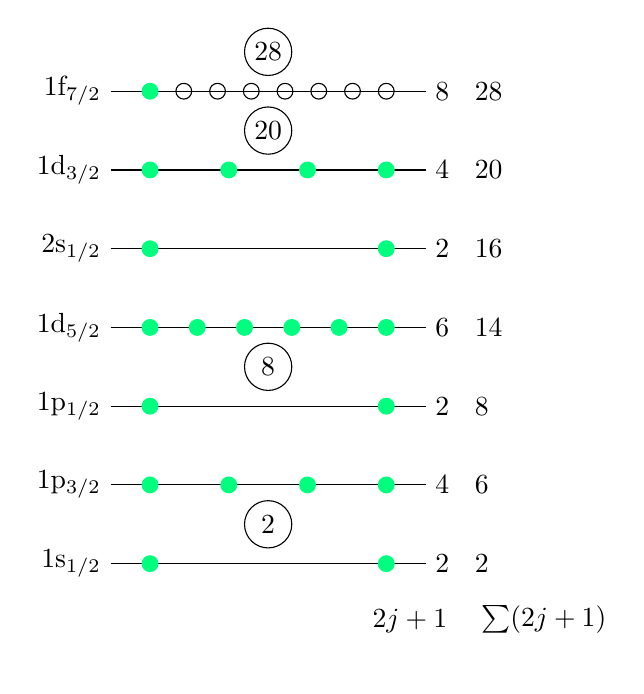
\begin{tikzpicture}[baseline=(current bounding box.center)]
        % Energy levels
        \node[anchor=south, label={$2j + 1$}, minimum size=8pt] at (3.8, -1.3) {};
        \node[anchor=south, label={$\sum(2j + 1$)}, minimum size=8pt] at (5.5, -1.3) {};

        \foreach \y/\label/\neutrons/\numberlabel in {0/1s$_{1/2}$/2/2, 1/1p$_{3/2}$/4/6, 2/1p$_{1/2}$/2/8, 3/1d$_{5/2}$/6/14, 4/2s$_{1/2}$/2/16, 5/1d$_{3/2}$/4/20, 6/1f$_{7/2}$/8/28} {
            \draw (0,\y) -- (4,\y);
            \node[anchor=east] at (0,\y) {\label};
            \node[anchor=west] at (4,\y) {\neutrons};
            \node[anchor=west] at (4.5, \y) {\numberlabel};
        }

        % Magic number
        \foreach \y/\magic in {0.5/2, 2.5/8, 5.5/20, 6.5/28} {
            \node at (2, \y) [circle,draw, label={[label distance=-0.2cm]center:\magic}, minimum size=0.6cm] {};
        }
        
        % Neutrons filled states
        \foreach \y/\capacity in {0/2, 1/4, 2/2, 3/6, 4/2, 5/4} {
            \ifnum\y=0
                \foreach \x in {1,2} {
                    \filldraw[pinkwave] ({(\x - 1) * (3.5 - 0.5) / (\capacity - 1) + 0.5}, \y) circle (0.1);
                }
            \else
                \foreach \x in {1,...,\capacity} {
                    \filldraw[pinkwave] ({(\x - 1) * (3.5 - 0.5) / (\capacity - 1) + 0.5}, \y) circle (0.1);
                }
            \fi
        }

        \foreach \x in {1} {
            \filldraw[pinkwave] ({(\x - 1) * (3.5 - 0.5) / (8 - 1) + 0.5}, 6) circle (0.1);
        }

        % Neutrons empty states
        \foreach \x in {2,...,8} {
            \draw ({(\x - 1) * (3.5 - 0.5) / (8 - 1) + 0.5}, 6) circle (0.1);
        }
    \end{tikzpicture}
\end{document}
